
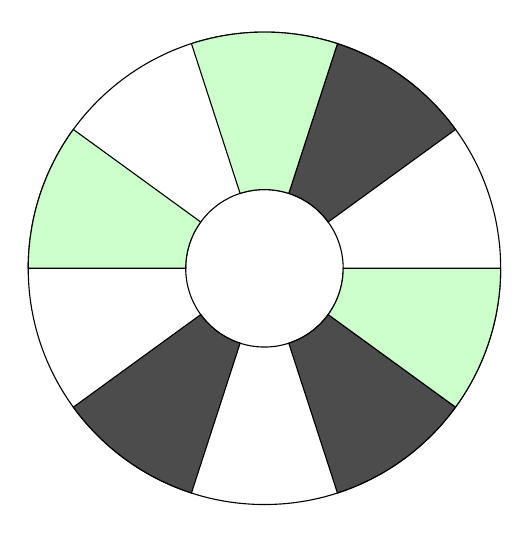
\begin{tikzpicture}
\filldraw[fill=white,draw=black](0,0)circle(1)(0,0)circle(3);
\filldraw[fill=gray!60!black,draw=black]
(72:1)arc(72:36:1)--(36:3)arc(36:72:3)--cycle
(216:1)arc(216:252:1)--(252:3)arc(252:216:3)--cycle
(288:1)arc(288:324:1)--(324:3)arc(324:288:3)--cycle;
\filldraw[fill=green!20!white,draw=black]
(72:1)arc(72:108:1)--(108:3)arc(108:72:3)--cycle
(144:1)arc(144:180:1)--(180:3)arc(180:144:3)--cycle
(0:1)arc(360:324:1)--(324:3)arc(324:360:3)--cycle;
\end{tikzpicture}

Note: diagram is \textbf{NOT} to scale.

In the diagram above, the shaded regions are congruent sectors of a donut shape that comes from removing a circle of radius $1$ from a concentric circle of radius $3$.  If a point is selected at random within this diagram, what is the probability it lands in a shaded region?



\ifsat
	\begin{enumerate}[label=\Alph*)]
		\item $\frac{8}{15}$%
		\item $\frac{6}{11}$
		\item $\frac{5}{9}$
		\item $\frac{3}{5}$
	\end{enumerate}
\else
\fi

\ifacteven
	\begin{enumerate}[label=\textbf{\Alph*.},itemsep=\fill,align=left]
		\setcounter{enumii}{5}
		\item $\frac{8}{15}$%
		\item $\frac{6}{11}$
		\item $\frac{5}{9}$
		\addtocounter{enumii}{1}
		\item $\frac{3}{5}$
		\item $\frac{4}{9}$
	\end{enumerate}
\else
\fi

\ifactodd
	\begin{enumerate}[label=\textbf{\Alph*.},itemsep=\fill,align=left]
		\item $\frac{8}{15}$%
		\item $\frac{6}{11}$
		\item $\frac{5}{9}$
		\item $\frac{3}{5}$
		\item $\frac{4}{9}$
	\end{enumerate}
\else
\fi

\ifgridin
 $\frac{8}{15}$%
		
\else
\fi

